% Number 160
% CVPMA Algebra Units Prefixes
% Problem-solving, Nostromo signal - hard!
% JG

% Watermark
\AddToShipoutPicture*{\BackgroundPic}

\addtocounter {ProbNum} {1}

%\begin{floatingfigure}[r]{.3\textwidth}
%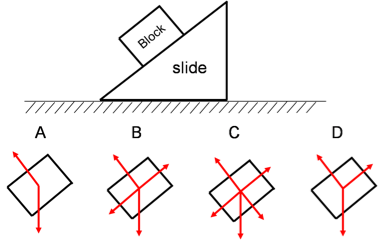
\includegraphics[scale=.4]{/Users/jgates/desktop/latex/pics/incline3.png}
%\end{floatingfigure}
 
{\bf \Large{\arabic{ProbNum}}} As its crew sleeps, the Nostromo glides through space at a brisk clip of ${920~\tfrac{km}{s}}$, relative to a nearby asteroid that it is approaching.  The computer uses radar (object detection using radio waves, which travel at the speed of light: ${3 \times 10^8 ~\tfrac{m}{s}}$) to detect objects in the ship's path.  The radio waves are emitted by the ship, bounce off of the asteroid, and return to the ship, where the computer analyzes the results.

\bigskip
Assume that the asteroid begins at the limit of the ship's effective radar range of 2 million km.  Once it detects the asteroid, the computer will require 15 minutes to revive the crew.  

\bigskip

How much time will the crew have to turn the ship at that point?
%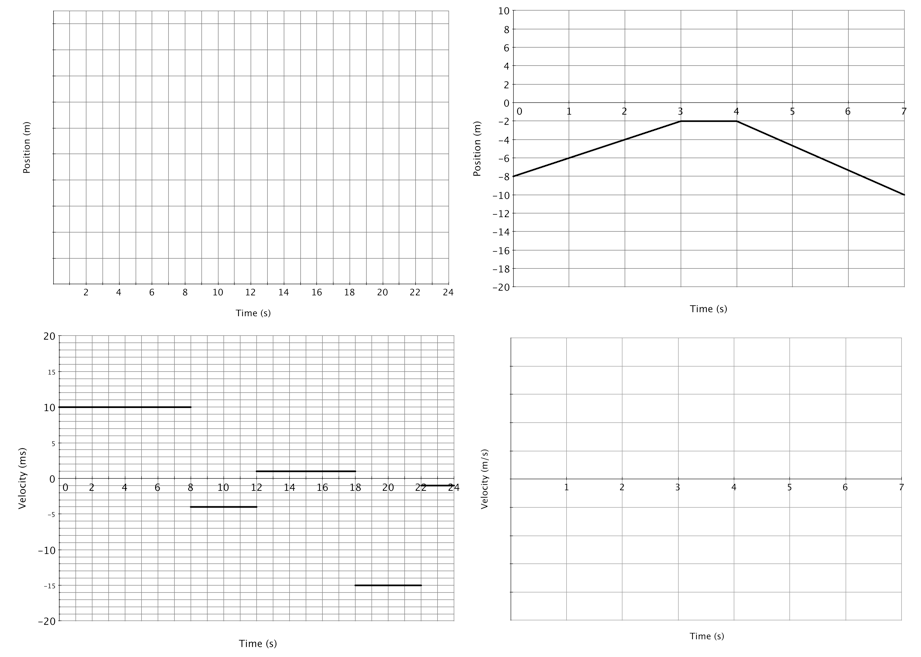
\includegraphics[scale=.57]{/Users/jgates/desktop/latex/pics/cvpmgraphs1.png}

\vfill

\newpage
